\subsection{Off-source data scenario}
\label{app:expo}
As described in the main text, we follow the strategy outlined in Ref. \cite{Coronado_Blazquez_2021} to extrapolate MAGIC observations to CTAO. 
The distribution of MAGIC pointings, that we consider when extrapolating the observation time and pointing directions of future CTAO measurements across the sky, is shown in \cref{fig:expo_dist}, together with one realization of the predicted CTAO distributions of the same quantities, i.e. the Galactic latitude, longitude, and the observation time per pointing. The distribution of the cumulative pointing time over all pointings, obtained from 1000 different realizations of future CTAO observations, is shown in \cref{fig:expo}.
\begin{figure*}
    \centering
    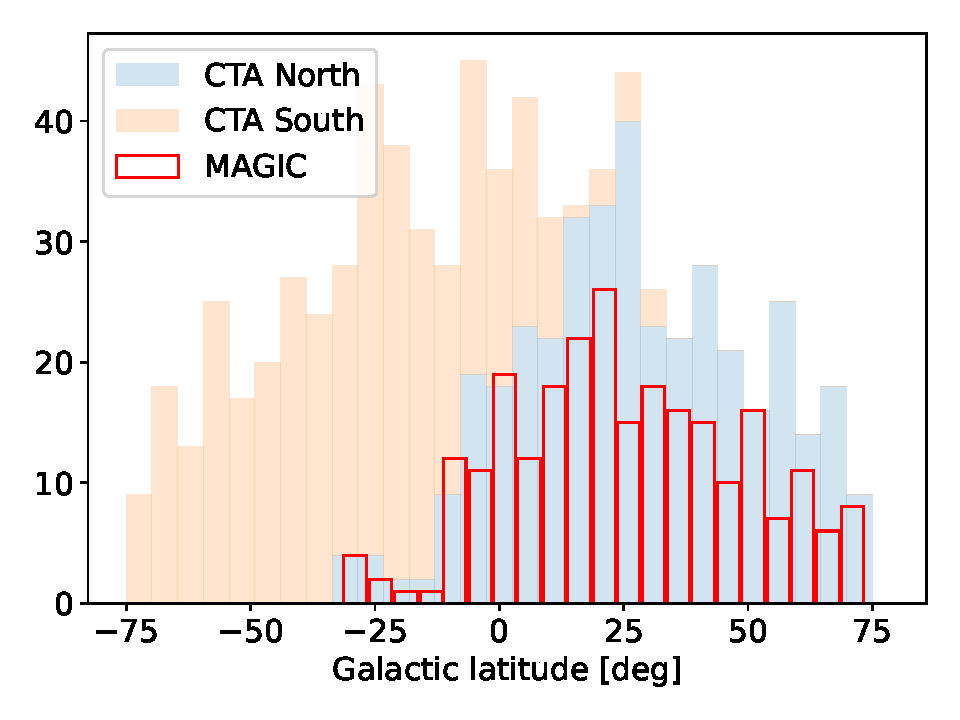
\includegraphics[width=0.32\textwidth]{paper_xcorr/figures/previous_analysis/distribution_DEC.pdf}
    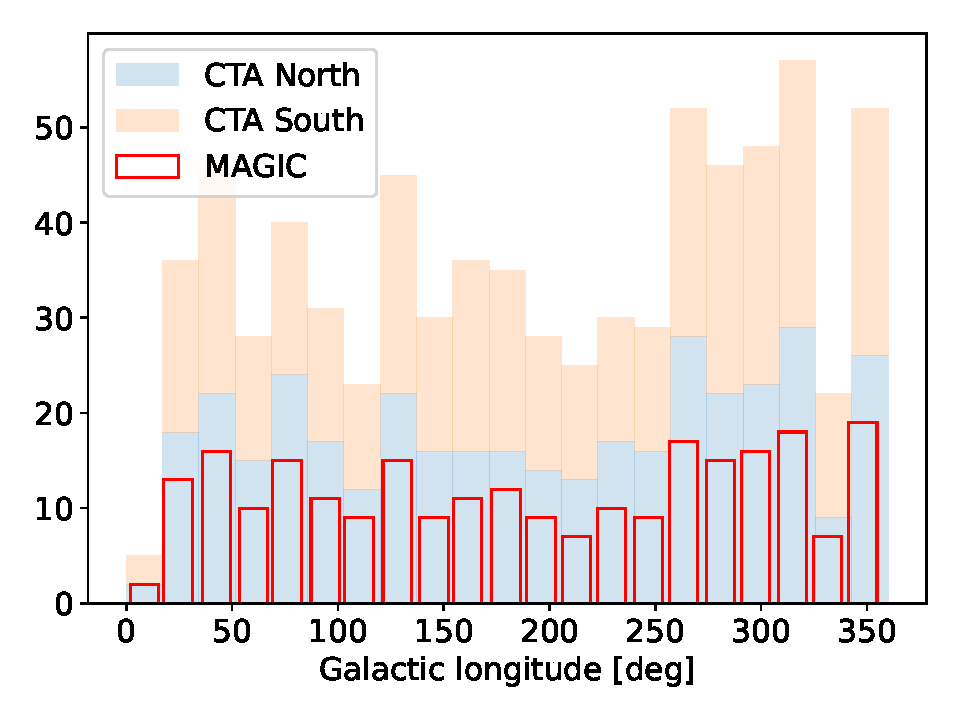
\includegraphics[width=0.32\textwidth]{paper_xcorr/figures/previous_analysis/distribution_RA.pdf}
    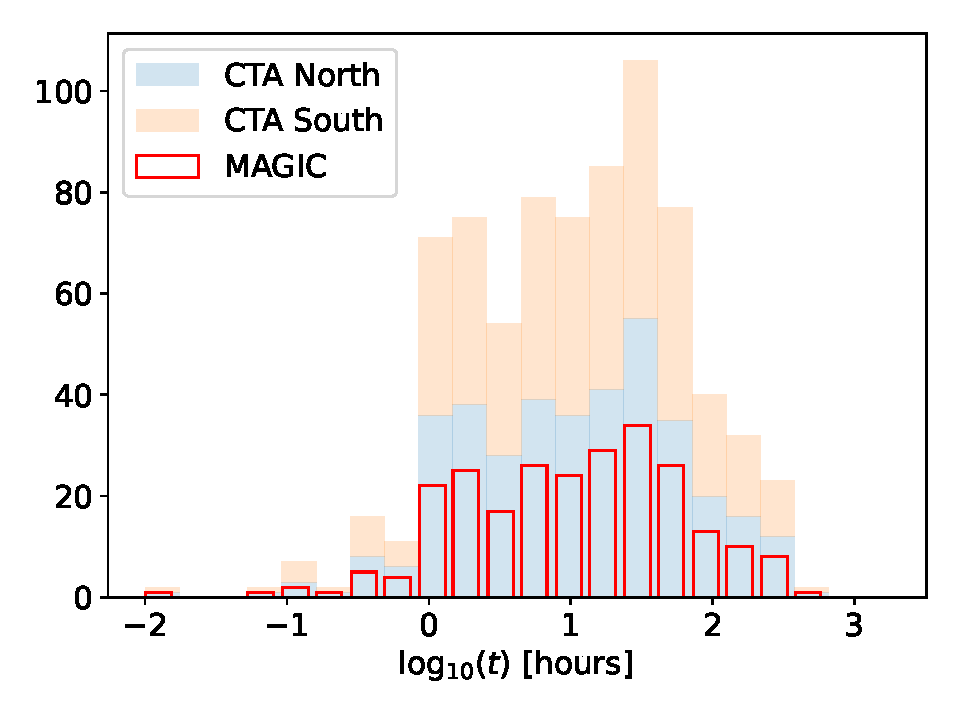
\includegraphics[width=0.32\textwidth]{paper_xcorr/figures/previous_analysis/distribution_time.pdf}   
    \caption{Distributions of Galactic latitude (left), longitude (center), and observation time (right) for one realization of the predicted CTAO pointings over 10 years of observations. The stacked histograms show contributions from the Northern (blue) and Southern (orange) arrays. For comparison, the red outlined histograms indicate the corresponding distributions from 6.5 years of MAGIC observations.}
    \label{fig:expo_dist}
\end{figure*}

\begin{figure}[t!]
    \centering
    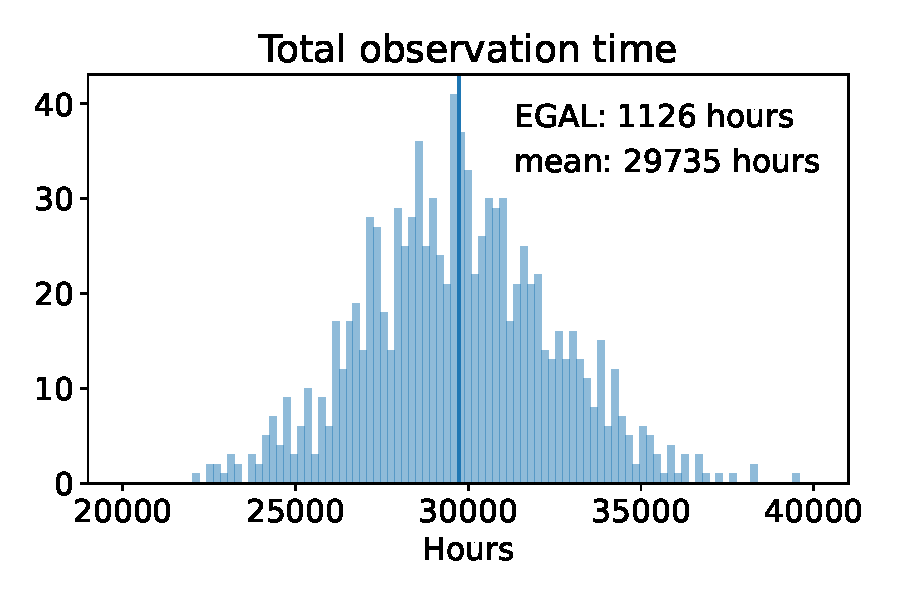
\includegraphics[width=0.45\textwidth]{paper_xcorr/figures/previous_analysis/average_time.pdf}
    \caption{Distribution of the total observation time from 1000 realizations of predicted CTAO pointings across the whole sky using both arrays. The blue vertical line marks the mean total observation time. {The total time in the most optimistic scenario is about 25 times higher than that of the EGAL survey, effectively translating the nominal 3 hours per pointing into $\sim 50$ hours per sky location in this scenario.} }
    \label{fig:expo}
\end{figure}

